\subsection{Network and observation campaign}
\label{sec:results-network}

\begin{figure}[t]
  \centering
  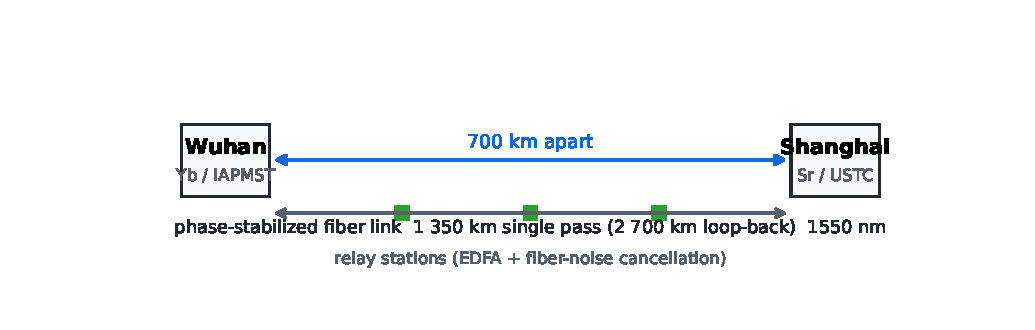
\includegraphics[width=\linewidth]{figs/fig1_network.pdf}
  \caption{The two-clock network. An IAPMST ytterbium clock in Wuhan and
  a USTC strontium clock in Shanghai are connected by a phase-stabilized
  \qty{1550}{nm} fiber link. Relay stations along the route carry
  erbium-doped fiber amplifiers and fiber-noise-cancellation loops.}
  \label{fig:network}
\end{figure}

Figure~\ref{fig:network} shows the two-clock network. An ytterbium (Yb)
lattice clock at IAPMST in Wuhan (systematic uncertainty
$\uYbE\times10^{-18}$~\citep{zhu2026yb}) and a strontium (Sr) lattice
clock at USTC in Shanghai ($\uSrE\times10^{-18}$~\citep{jia2026sr}) are
separated by $\siteKm$\,km and compared through a $\fibreKm$\,km
phase-stabilized fiber link ($\roundKm$\,km loop-back), with the
carrier transmitted from Shanghai to Wuhan on a \qty{1550.12}{nm}
telecom channel. The link extends the field-deployed link of
ref.~\citep{chen2026dissemination}, using the same cascaded
fiber-noise-cancellation technique; its added instability stays below
the clock noise for averaging times beyond $100$\,s.

Both combs are self-referenced and phase-locked to the local clock
signal, and all other frequencies in the chain derive from the two
clock transitions through fixed factor-of-two relations
(698/1397 nm on the Sr side; 578/1156 nm on the Yb side), so the two
clocks are the system's only independent frequency sources. The
recorded quantity is the out-of-loop beat between the received carrier
and the local Yb-referenced comb, sampled every second and converted to
fractional units with $F_{1550} = \fFifteenTHz$\,THz; the fiber
loop-back is monitored out of loop throughout. Each retained segment
yields a frequency-ratio estimate through the fixed frequency-chain
relations (see Methods).

Over two months (\nDays~days, \nStages~stages) the two clocks and their
transfer chains ran synchronously for a total of \nSamplesAll~valid
seconds, recorded as \nSegAll~jump-free segments; the data set analyzed
here comprises \nSeg~segments with \nSamples~seconds
(\nHours~effective hours). Figure~\ref{fig:campaign}a places the
segments on the campaign timeline.

\subsection{Clock-ratio determination}
\label{sec:results-ratio}

\begin{figure}[t]
  \centering
  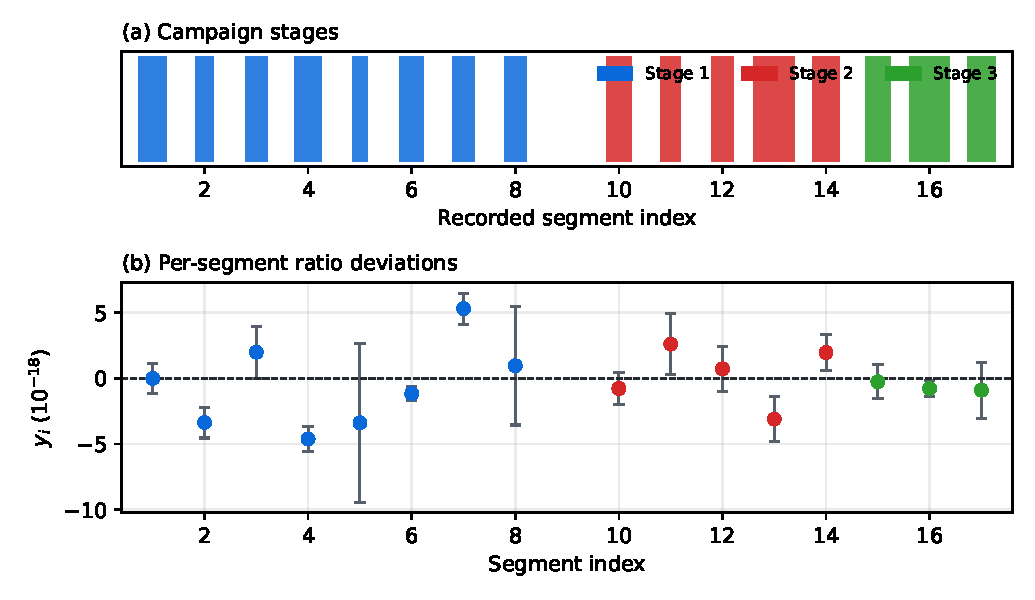
\includegraphics[width=\linewidth]{figs/fig2_campaign.pdf}
  \caption{Campaign and per-segment data. (a) Recorded segments colored
  by measurement stage; bar widths scale with the square root of the
  retained sample count. (b) Per-segment ratio deviations $y_i$ with
  their statistical uncertainties; the dashed line marks zero deviation.}
  \label{fig:campaign}
\end{figure}

We determine the Yb/Sr frequency ratio from the \nSeg~segments. Each
segment yields a ratio estimate with its own statistical uncertainty
estimated from the Allan deviation of the beat
(Methods). The segment estimates scatter more
than their individual uncertainties allow: the fixed-effect weighted
least-squares fit gives $\chi^2_{\rm red} = \chiRed$ for
$\dofV$ degrees of freedom ($p = \pChi$), and
\nModelLimited~of the \nSeg~segments have stability fits that fall
outside the white-frequency-noise band (groups \modelLimitedGroups).
We therefore adopt the Bayesian random-effect estimate, which treats
the excess scatter as a free parameter and propagates its posterior
uncertainty, while the fixed-effect WLS and Mandel--Paule estimates are
kept as cross-checks.

The resulting Yb/Sr ratio is
\begin{equation}
  \mathrm{Yb/Sr} = \Rheadline(\RheadlineUnc),
\end{equation}
with a statistical uncertainty of
$\uStatShort\times10^{-18}$ and a total standard uncertainty of
$\uTotalShort\times10^{-18}$ (Section~\ref{sec:results-budget}). The
precision-weighted cross-checks agree within their uncertainties:
the WLS center is \RwlsHead\xspace and the Mandel--Paule center is
\RmpHead\xspace (rounded at the 19th decimal), both consistent with
the adopted value at the $10^{-18}$ level. Figure~\ref{fig:campaign}b shows the per-segment
deviations; the segment-to-segment scatter is dominated by the
statistical noise of the individual segments and by the excess scatter
captured by the random-effect term.

\subsection{Uncertainty budget}
\label{sec:results-budget}

Table~\ref{tab:budget} collects the components of the total standard
uncertainty (Figure~\ref{fig:compare}b). The statistical term dominates
the budget, followed by the Yb and Sr systematic evaluations, the
static-potential term from the leveling, and the time-varying-redshift
term carried as an uncertainty item; the fiber-link and comb terms are
negligible at this precision. The total standard uncertainty is
$\uTotalShort\times10^{-18}$.

\begin{table}[t]
  \centering
  \caption{Uncertainty budget of the Yb/Sr frequency-ratio
  measurement. The time-varying gravitational-redshift term is carried
  as an uncertainty item and is not applied as a correction to the
  central value. Components are treated as independent.}
  \label{tab:budget}
  \begin{tabular}{lS[table-format=1.3]}
    \toprule
    Component & {Contribution ($10^{-18}$)} \\
    \midrule
    Statistical (Bayesian random effect) & \uStatE \\
    Sr systematics                       & \uSrE \\
    Yb systematics                       & \uYbE \\
    Static gravitational potential       & \uStaticE \\
    Fiber link                           & \uLinkE \\
    Frequency comb                       & \uCombE \\
    Time-varying redshift                & \uTidalE \\
    \midrule
    Total (quadrature)                   & \uTotalE \\
    \bottomrule
  \end{tabular}
\end{table}
